\documentclass{math}

\usepackage{tikz}

\title{CSCI 251: Concepts of Parallel and Distributed Systems}
\author{Alvin Lin}
\date{November 27th, 2017}

\begin{document}

\maketitle

\section*{Networking}
Topics:
\begin{itemize}
  \item Circuit Switching
  \item Packet Switching
\end{itemize}

\subsection*{Circuit Switching}
\begin{center}
  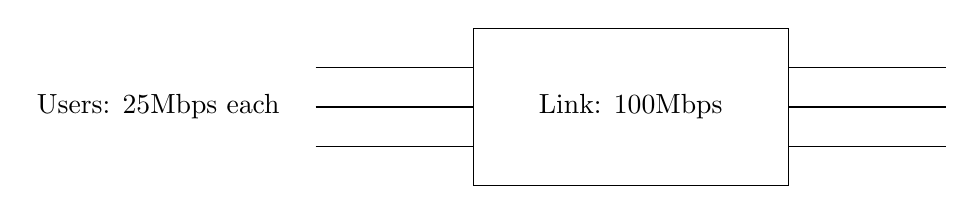
\begin{tikzpicture}
    \draw (0,0) -- (4,0) -- (4,2) -- (0,2) -- cycle;
    \node at (2,1) {Link: 100Mbps};
    \draw (-2,0.5) -- (0,0.5);
    \draw (-2,1) -- (0,1);
    \draw (-2,1.5) -- (0,1.5);
    \node[fill=none] at (-4,1) {Users: 25Mbps each};
    \draw (4,0.5) -- (6,0.5);
    \draw (4,1) -- (6,1);
    \draw (4,1.5) -- (6,1.5);
  \end{tikzpicture}
\end{center}
The maximum number of users that can be supported is 4 users, each with a
dedicated connection.

\subsection*{Packet Switching}
In the same scenario, if the number of users is \( N \) and each user is
transmitting for 30\% of the time \( p = 0.3 \), then the probability of a
given user transmitting and all other users not transmitting is:
\[ p^1(1-p)^{n-1} \]
The probability of any user transmitting and the rest not transmitting:
\[ \binom{N}{1}p^1(1-p)^{n-1} \]
The probability of \( k \) users transmitting and the rest not transmitting:
\[ \binom{N}{k}p^k(1-p)^{n-k} \]

\subsection*{Delays}
Suppose we are transmitting packets of size \( L \) Mbits at a transmission rate
of \( R \) Mbits per second with a delay \( d = \frac{L}{R} \) seconds. The
number of packets that can be transmitted every seconds is \( \frac{1}{d} \).
Delays can result from queueing, transmission, processing, and propagation.
Propagation delay is usually defined by the speed of light, which is the speed
at which packets are transmitted through wires.

\subsection*{Mobility}
Wireless networks are networks with low mobility, while cellular networks have
high mobility. We can let the routing hardware handle the mobility or have the
end systems handle mobility. The former is much more expensive and not scalable.
\begin{center}
  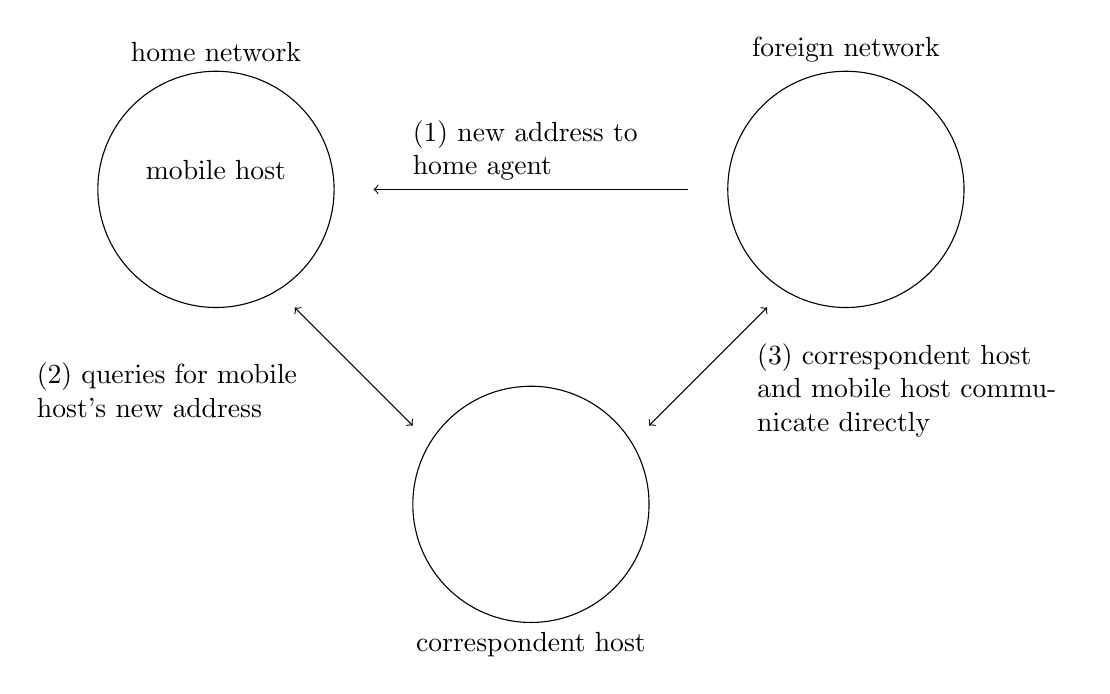
\begin{tikzpicture}
    \node[above] at (0,0) {mobile host};
    \draw (0,0) circle (1.5cm) node[above,yshift=1.5cm] {home network};
    \draw (8,0) circle (1.5cm) node[above,yshift=1.5cm] {foreign network};
    \draw (4,-4) circle (1.5cm) node[below,yshift=-1.5cm] {correspondent host};
    \draw[->] (6,0) -- (2,0) node[pos=0.5,above,text width=3cm]
      {(1) new address to home agent};
    \draw[<->] (2.5,-3) -- (1,-1.5)
      node[pos=0.3,left,text width=4cm,xshift=-0.2cm]
      {(2) queries for mobile host's new address};
    \draw[<->] (5.5,-3) -- (7,-1.5)
      node[pos=0.3,right,text width=4cm,xshift=0.8cm]
      {(3) correspondent host and mobile host communicate directly};
  \end{tikzpicture}
\end{center}

\section*{Reminders}
Work on Project 2.

\noindent Professor Mohan Kumar: \\
\url{mjkvcs@rit.edu} \\
\url{https://cs.rit.edu/~mjk} \\

\noindent Rahul Dashora (TA): \\
\url{rd5476@mail.rit.edu} \\

\begin{center}
  You can find all my notes at \url{http://omgimanerd.tech/notes}. If you have
  any questions, comments, or concerns, please contact me at
  alvin@omgimanerd.tech
\end{center}

\end{document}
